\documentclass[11pt,a4paper]{article}
\usepackage{fontspec}
\setmainfont{TeX Gyre Pagella}
\newfontfamily\headfont{Inter}[UprightFont=*-ExtraBold,BoldFont=*-ExtraBold,Extension=.otf,Path=/usr/share/fonts/opentype/inter/]
\usepackage[a4paper,margin=2.3cm]{geometry}
\usepackage{graphicx,booktabs,float,caption,array,xcolor,longtable}
\usepackage{xurl}
\usepackage[hidelinks]{hyperref}
\usepackage{titlesec}
\usepackage[round]{natbib}
\usepackage{setspace}
\setstretch{1.05}
\renewcommand{\topfraction}{0.9}
\renewcommand{\bottomfraction}{0.8}
\renewcommand{\textfraction}{0.1}
\renewcommand{\floatpagefraction}{0.75}
\setlength{\parindent}{0pt}
\setlength{\parskip}{0.55em}
\titleformat{\section}{\headfont\Large}{\thesection}{0.8em}{}
\titleformat{\subsection}{\headfont\large}{\thesubsection}{0.8em}{}
\captionsetup{font=small,labelfont=bf}
\urlstyle{same}
\hypersetup{pdftitle={When Did Your Country Lose 11 Days?},pdfauthor={Tristan Hotham}}

\begin{document}
\begin{center}
{\Large\bfseries When Did Your Country Lose 11 Days?\par}
\vspace{0.4em}
{\large Four great switches, from the Gregorian calendar to votes for women,\\country by country in Wikipedia's tables, 1582 to 2026\par}
\vspace{1.2em}
{\large Tristan Hotham\par}
\vspace{0.3em}
{\small Independent researcher\\
ORCID: 0000-0003-4931-9349\\
DOI: https://doi.org/10.5281/zenodo.23873009\par}
\vspace{0.8em}
2026
\end{center}

\begin{quote}
\small
\begin{center}\textbf{Abstract}\end{center}
I map four switches that most of the world made over the last four and a half centuries: from the Julian to the Gregorian calendar, from one side of the road to the other, to the metric system, and to votes for women. The dates come from the tables and prose of 19 English Wikipedia articles, read cell by cell and matched to today's 197 countries, with sub-national detail where the sources give it. For the calendar the primary source is Wikipedia's list of 146 historic areas with their switch dates; with the other tables it dates the switch for 82 of today's countries (27 of them through the colonial power that then ruled them), from Catholic Europe in 1582 to Saudi Arabia's civil switch in 2016, 434 years later. Parts of 45 countries dropped 10 dates, of 19 dropped 11 (among them Britain and its colonies in 1752), of two (Switzerland and Uganda) dropped 12 and of 19 dropped 13; 11 came from other calendars, four have never adopted it, and the list records 8 returns to the Julian calendar. The driving table records 62 countries changing side at a known date, 59 to the right and 3 to the left; the busiest decade was the 1920s, and today 54 countries, home to 35.6\% of the world's people, drive on the left. Official metrication started in France in 1795 and, in the table, last in Samoa in 2015; the median start is 1920, and five countries are listed as still using non-metric units officially. Women could first vote nationally in New Zealand in 1893; half of today's countries had followed by 1951, and the last was Saudi Arabia, in municipal elections, in 2015. For 18 countries the table separates a restricted first vote from a later vote on equal or full terms, up to 65 years apart. Each switch came in waves, set by religion, empire, war and independence, and each left stragglers.

\textbf{Keywords:} Gregorian calendar; calendar reform; driving side; metrication; women's suffrage; diffusion; standardisation; historical geography; Wikipedia; open data
\end{quote}

\section{Introduction}
Some of the most ordinary features of modern life, the date, the side of the road, the kilogram and the ballot, were once settled differently in each country and are now nearly universal. Each became universal through a sequence of national decisions spread over decades or centuries. This paper assembles, from openly licensed sources, the year in which each of today's countries made four such switches, and maps them together on an interactive page (\url{https://maps.tristanhotham.com/calendar-switch/}). The aim is descriptive: to show the waves in which each switch spread, the first and last to move, the places that went back and forth, and how much the record depends on what the sources choose to tabulate.

The four switches differ in kind. The calendar change was a technical correction promulgated by a pope in 1582 and adopted by civil authorities as religion and politics allowed. The side of the road is a pure coordination problem, with no better answer, where neighbours, empires and vehicle imports decide. Metrication is a standard adopted by law and then, sometimes, abandoned in practice. Votes for women are a question of rights, extended in steps and sometimes withdrawn.

\section{Data}
All the dates come from English Wikipedia, saved in 2026 with their revision numbers (Table~\ref{tab:revs}) \citep{wiki}. For the calendar the primary source is the table in "List of adoption dates of the Gregorian calendar by country" (146 rows, each a historic area within one of 51 present countries, giving the year, the last day before and the first day after the change, the number of dates omitted, negative for a return to the Julian calendar, and notes), the per-country list to which "Adoption of the Gregorian calendar" points. I cross-check it against the "Adoption by country" table in "Gregorian calendar" (20 rows of a year and the countries or areas that adopted the calendar in it), the tables of the start of the numbered year in "Gregorian calendar" and "Julian calendar" (16 and 16 rows), and the country by country prose of "Adoption of the Gregorian calendar". "Calendar (New Style) Act 1750" and "Old Style and New Style dates" supply the British details. For driving I use the table "Worldwide distribution by country" in "Left- and right-hand traffic" (231 rows: country, side, date of switch, notes) and its prose, with "Dagen H" for Sweden. For metrication I use the status table in "Metrication" (77 rows: the year the official metrication process started, the previous system and the current status). For votes I use the table in "Women's suffrage" (199 rows: the year women first won the vote at national level and notes). Other articles listed in Table~\ref{tab:revs} were read for context; one requested article, a list of countries by date of decimal currency, does not exist. Country outlines and sub-national units are Natural Earth's \citep{naturalearth}.

\section{Methods}
\subsection{Reading the tables}
Every table was read cell by cell with row and column spans expanded and footnote markers removed; "citation needed" tags were kept as a flag. The parsed tables are published unchanged in \texttt{data/source\_tables/}. The build stops if a table changes size or a quoted sentence disappears from its page.

\subsection{Today's countries and stand ins}
Each row is matched by name to one of today's 197 countries: the Natural Earth units that are their own sovereign, which gives the 193 United Nations members with Vatican City, Taiwan, Kosovo and Palestine. Dependencies are drawn where a table gives them a row but are not counted. The list article already assigns each historic area to a present country. Elsewhere a historical state is drawn with the modern country covering most of it, and each such case is recorded as a stand in: Yugoslavia with Bosnia and Herzegovina and Kosovo for the calendar, the Papal States with Vatican City, the Commonwealth's lands with Ukraine in the prose, and, for votes, Czechoslovakia, Yugoslavia, the British Leeward and Windward Islands and the two Yemens with their successors. Sub-national units come from Natural Earth's states and provinces where the sources name them: for the calendar the Dutch and Belgian provinces, 22 Swiss cantons, Alsace and Lorraine (drawn as French departments), Quebec (New France), Nova Scotia and Alaska; the Canadian provinces, the Austrian states and Okinawa for driving; the Swiss cantons for metrication and votes; and the Canadian provinces and Australian states for votes at those levels.

\subsection{The calendar}
Each row of the list is dated by its first new style day, so 21 December 1585 followed by 1 January 1586 counts as 1586. A country with a single date gets that year. For the 16 countries whose rows differ I build a timeline by hand from the rows (the code's \texttt{polities.py}), keeping the parts that switched early, the returns to the Julian calendar, the Swedish calendar of 1700 to 1712 and the French Republican calendar of 1793 to 1805. A country's calendar year is the start of the last unbroken period in which the whole of today's country was Gregorian (the Republican interlude, a different reform, does not break it); the first year any part switched is kept as well. Alaska, which was Russian until 1867, is drawn separately rather than holding back the United States. Where the list and the other sources differ (Table~\ref{tab:dis}) I keep the list and report the other. For countries not in the list I use the adoption tables and prose. The adoption table's 1582 row covers Spain, Portugal, France and others "and colonies thereof", and its 1752 row "the First British Empire"; the list has Spanish, Portuguese and British Empire rows; and the article adds that the colonies of the Americas changed when their mother countries did. I therefore date 27 former colonies by the power that ruled them at the time (the Spanish and Portuguese Americas and the Philippines in 1582; Britain's Caribbean colonies in 1752). This mapping is mine and is marked on the map. The 111 countries the sources do not name are not missing from the calendar: the article says the Gregorian calendar is now the sole civil calendar of the vast majority of countries. They simply have no date here.

The days dropped are the list's number of dates omitted. Every positive value matches the rule in the "Gregorian calendar" article's table of ranges (10 days for a first new style day before March 1700, 11 to February 1800, 12 to February 1900, 13 thereafter), except Alaska, where the date line moved as well and 11 dates were omitted instead of 12. Note that a switch on 1 March 1700, as in Denmark-Norway and the Protestant German states, omits 11 dates, the old calendar's 29 February 1700 among them. A country can have more than one value when its regions switched in different centuries (13 countries); for colonies and other countries not in the list the rule gives the value. Countries that came from other calendars have no dates dropped (Table~\ref{tab:days}).

\subsection{Driving side}
The driving year is the table's "date of switch". Before that date a country is shown on the other side. Where neither the table's notes nor the article describe the change (15 countries, including Belarus and Azerbaijan in 1966 and Denmark and Norway in 1793) the earlier years are flagged "date only". Where the table gives no date (135 countries) I assume today's side throughout; this is an assumption, and it inflates the share on the right in early years. I override the table where its own notes or the article give more: Timor-Leste (right 1928, left 1976), Uruguay (left 1918, right 1945), Suriname (a date of "1920s" but "did not switch sides"), Nauru (a date of 1918, but listed in the article among places that have always driven on the left), and countries where regions differed (Austria, Brazil, China, Spain, Italy, Romania, Canada).

\subsection{Metrication and votes}
The metric year is the year the table gives for the start of the official process, not its completion; Germany and Poland have a first year for part of today's country. For votes, a single year in the table is used as it stands. Where the year cell holds several years, I read it with the notes and keep the first year in which women could vote in national elections at all and, where given, the year of full or equal terms (Table~\ref{tab:votes}). Local, communal or cantonal votes are not counted as national, so Belgium's first year is 1948, not 1919; the Netherlands' is 1919, the year its notes give for voting, not 1917, the year women could be elected.

\subsection{Curves}
For each year from 1580 to 2026 I count today's countries in each state, and weight them by today's population (Natural Earth). The curves therefore describe how much of today's world had switched, not the share of people alive at the time.

\begin{table}[tbp]\centering\small\caption{Before and after dates in the sources (the list article, or the prose where it gives the weekday), and the dates omitted.}\label{tab:days}\begin{tabular}{p{3.6cm}p{9.2cm}r}\toprule Where & Switch & Days\\\midrule
Spain, Portugal & Thursday 4 October 1582 was followed by Friday 15 October 1582 & 10\\
Denmark and Norway & Sunday 18 February 1700 was followed by Monday 1 March 1700 & 11\\
Great Britain & Wednesday 2 September 1752 was followed by Thursday 14 September 1752 & 11\\
Sweden & Wednesday 17 February 1753 was followed by Thursday 1 March 1753 & 11\\
Uganda & 31 December 1893 was followed by 13 January 1894 & 12\\
Bulgaria & 31 March 1916 was followed by 14 April 1916 & 13\\
Russia & Wednesday 31 January 1918 was followed by Thursday 14 February 1918 & 13\\
Romania & 31 March 1919 was followed by 14 April 1919 & 13\\
Greece & Wednesday 15 February 1923 was followed by Thursday 1 March 1923 & 13\\
Albania & 14 November 1912 was followed by 28 November 1912 & 13\\
\bottomrule\end{tabular}\end{table}

\begin{table}[tbp]\centering\footnotesize\caption{Where the list article and the other calendar sources (adoption tables in Gregorian calendar and Julian calendar, and the prose of Adoption of the Gregorian calendar) differ. Most differences are finer regional detail in the list. Years are first part and whole country. GT: adoption table in Gregorian calendar; GN and JN: start of year tables in Gregorian calendar and Julian calendar; AG: Adoption of the Gregorian calendar; ACT: Calendar (New Style) Act 1750.}\label{tab:dis}\begin{tabular}{p{4.2cm}p{4.4cm}p{5.6cm}}\toprule Country or area & List & Other sources\\\midrule
Switzerland & 1583 to 1812 & 1584 to 1812 (AG; GT 1584 some Catholic Swiss cantons, 1700 some Protestant Swiss cantons)\\
Germany & 1582 to 1700 & 1583 to 1700 (GN; JN; AG; GT 1610 Prussia)\\
France & 1582 to 1760 & 1582 (GT 1582 France; AG)\\
Ireland & 1584 to 1752 & 1752 (GT 1752 Ireland; ACT)\\
Italy & 1582 to 1583 & 1582 (GT 1582 Italy; GN Papal States, Venice and Tuscany 1582)\\
Lithuania & 1586 to 1915 & 1582 to 1915 (GT 1582 Commonwealth, 1915 Lithuania; AG switch back in 1795)\\
Latvia & 1617 to 1915 & 1915 (GT 1915 Latvia)\\
Myanmar & 1885 & 1886 (AG Southeast Asia)\\
Poland & 1582 to 1700 & 1582 (GT 1582 Polish-Lithuanian Commonwealth; AG)\\
Romania & 1590 to 1919 & 1919 (GT 1919 Romania; AG)\\
Russia & 1610 to 1918 & 1918 (GT 1918 Russia; AG)\\
Turkey & 1917 & 1917 to 1926 (GT 1917 Ottoman Empire, 1926 Turkey; JN Ottoman Empire 1917; AG)\\
Ukraine & 1918 & 1582 to 1918 (AG Ukraine; GT 1918 Ukraine)\\
United States & 1582 to 1752 & 1752 (ACT, America; AG; GT 1752 First British Empire)\\
Ducal Prussia & 1610 & 1612 (AG); 1610 (GT) (AG)\\
Lithuania and Belarus, return to the Julian calendar & 1800 & 1795, after the Third Partition (AG) (AG)\\
Southern Netherlands (Belgium) & December 1582 & 1 January 1583 (AG) (AG)\\
Lorraine & 1582, back in 1735, again in 1760 & 1582 (GN), 1760 (JN) (GN; JN)\\
Alaska & Friday 6 October followed by Friday 18 October 1867 & Saturday 7 October followed by Friday 18 October (AG) (AG)\\
\bottomrule\end{tabular}\end{table}

\section{Results}
\subsection{Waves}
Figure~\ref{fig:curves} shows the four curves. The calendar moved in religious blocs: 33 of today's countries by 1600 (most of them colonies dated through Spain and Portugal), 49 by 1752 and 49 by 1800, then 73 by 1918 and 80 by 1950 as East Asia and the Orthodox east switched. Driving on the right, under my assumption for undated countries, went from 94 countries in 1900 to 126 in 1950 and 143 today. Metrication had started in 22 countries by 1875, 48 by 1950 and 60 by 1970. Votes for women spread fastest: 23 countries by 1918, 74 by 1945, 170 by 1970 and 195 today, the remaining two holding no elections.

\begin{figure}[tbp]\centering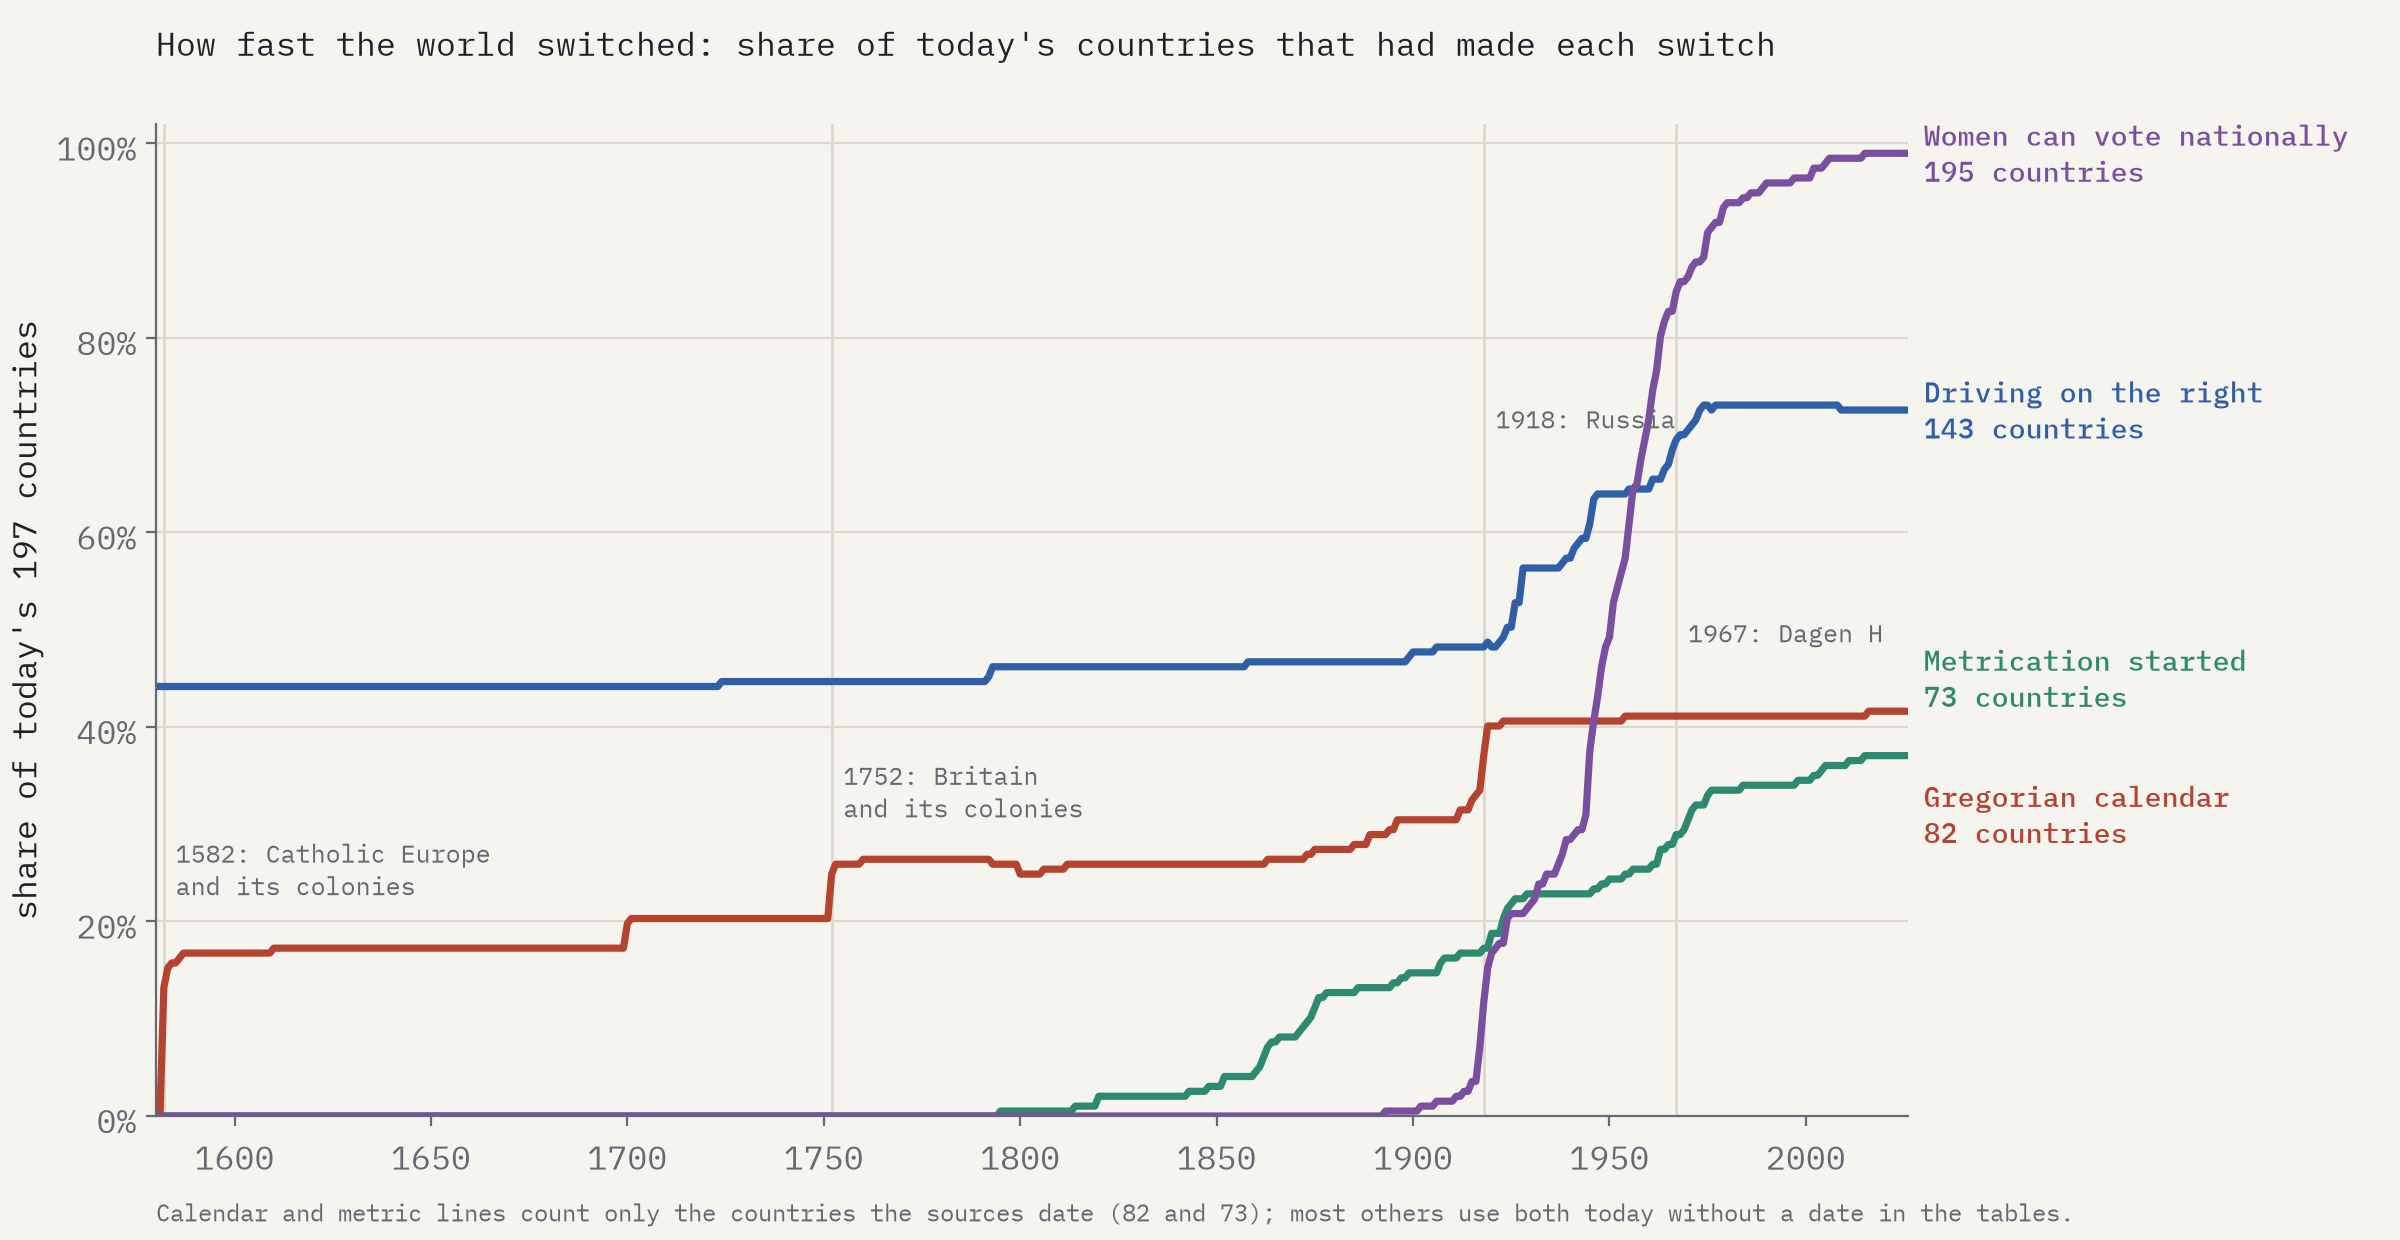
\includegraphics[width=\textwidth]{f_curves.png}
\caption{Share of today's countries that had made each switch, by year. Calendar and metric curves count only countries the sources date.}\label{fig:curves}\end{figure}

\subsection{The calendar}
Figure~\ref{fig:calmap} maps the calendar. Spain, Portugal, most of Italy and Poland switched on 4 to 15 October 1582, France (outside Alsace and Lorraine) and the Low Countries in December, Holland in January 1583, the Catholic German states, Austria and Slovenia in 1583, Bohemia, Moravia, Silesia and the Catholic Swiss cantons in 1584, the Grand Duchy of Lithuania in 1586, Hungary in 1587 and Transylvania in 1590. The Protestant German states, Denmark and Norway followed on 1 March 1700, the rest of the Dutch provinces and the Protestant Swiss cantons in 1700 and 1701, Britain and its colonies in September 1752 (9 of today's countries) and Sweden with Finland in 1753. Lorraine completed today's France in 1760; the last Swiss communes switched in 1812, and Uganda, under British rule, in 1894. Of the 22 countries the sources date to the twentieth century or later, most were in the Orthodox east and the Caucasus (1915 to 1923); the latest were Vietnam (1954) and Saudi Arabia (2016). Four countries have not adopted it: Afghanistan, Ethiopia, Iran and Nepal.

Figure~\ref{fig:days} counts the days dropped. The list records 8 returns to the Julian calendar: Groningen city (1594), Appenzell Ausserrhoden (1597), Nova Scotia under British rule (1710), Lorraine (1735), Courland (1796), the Lithuania Governorate (1800, covering parts of today's Lithuania and Belarus), the Swedish return of 1712 with its 30 February, and Ulster's Gaelic lordships, which had a papal dispensation to return by 1641. France replaced the Gregorian calendar with its Republican calendar from 1793 to the end of 1805. Each of these places later switched again.

\begin{figure}[tbp]\centering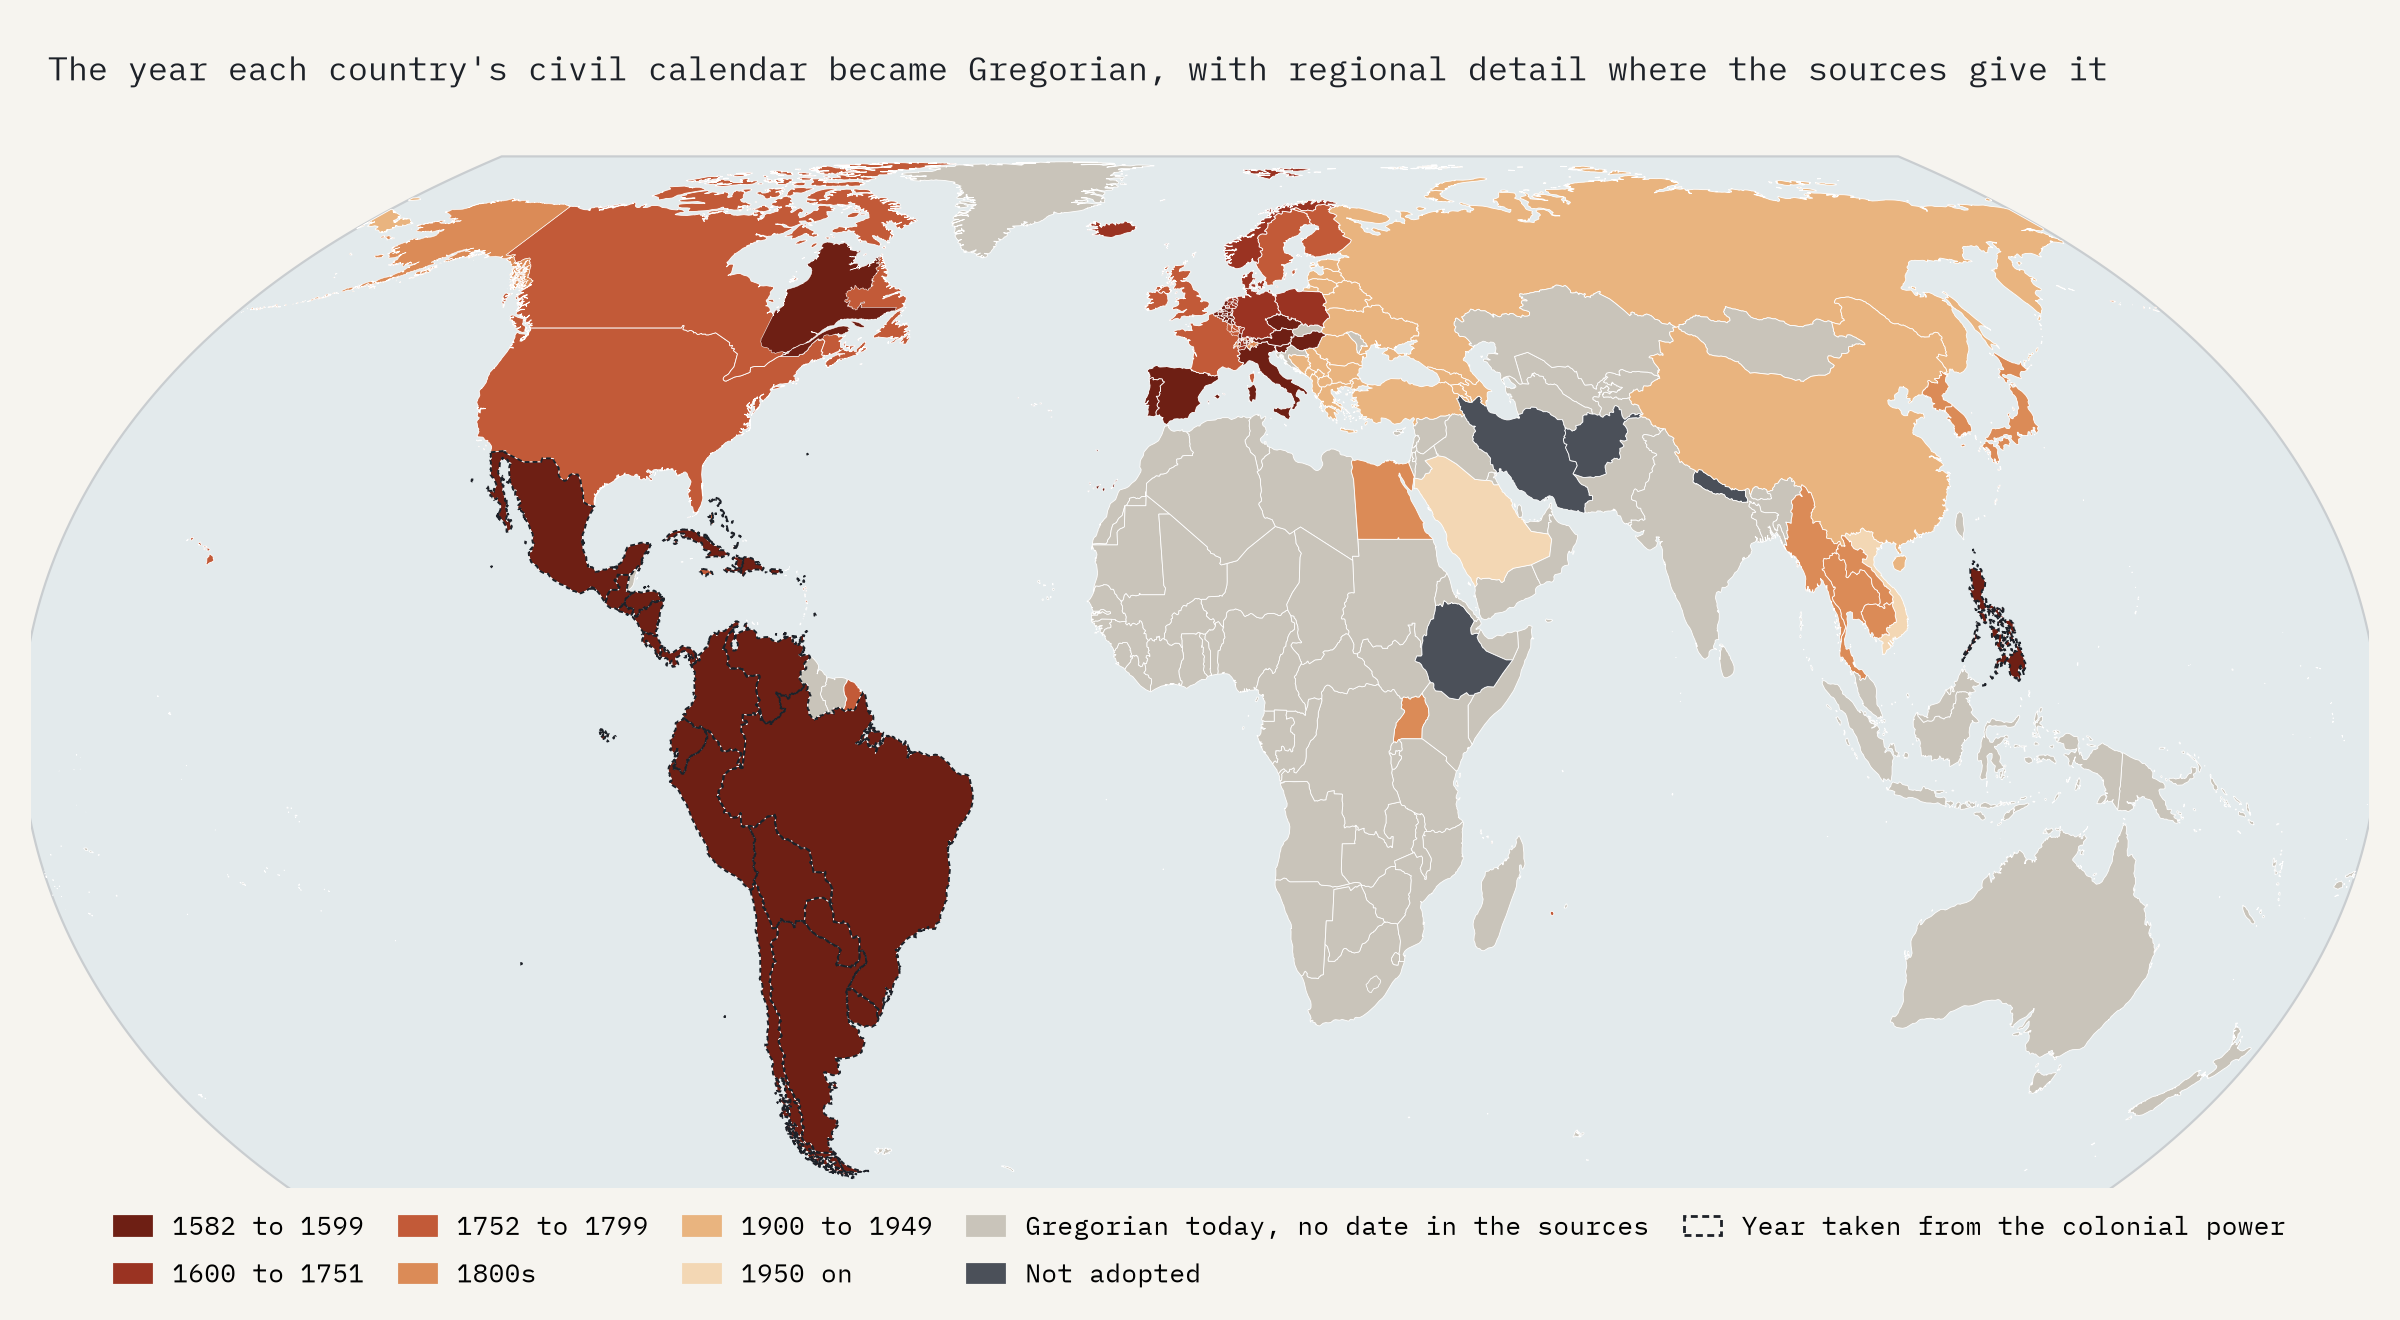
\includegraphics[width=\textwidth]{f_cal_map.png}
\caption{The year each country's civil calendar became Gregorian, with regional detail where the sources give it. Dashed outlines: years taken from the colonial power.}\label{fig:calmap}\end{figure}

\begin{figure}[tbp]\centering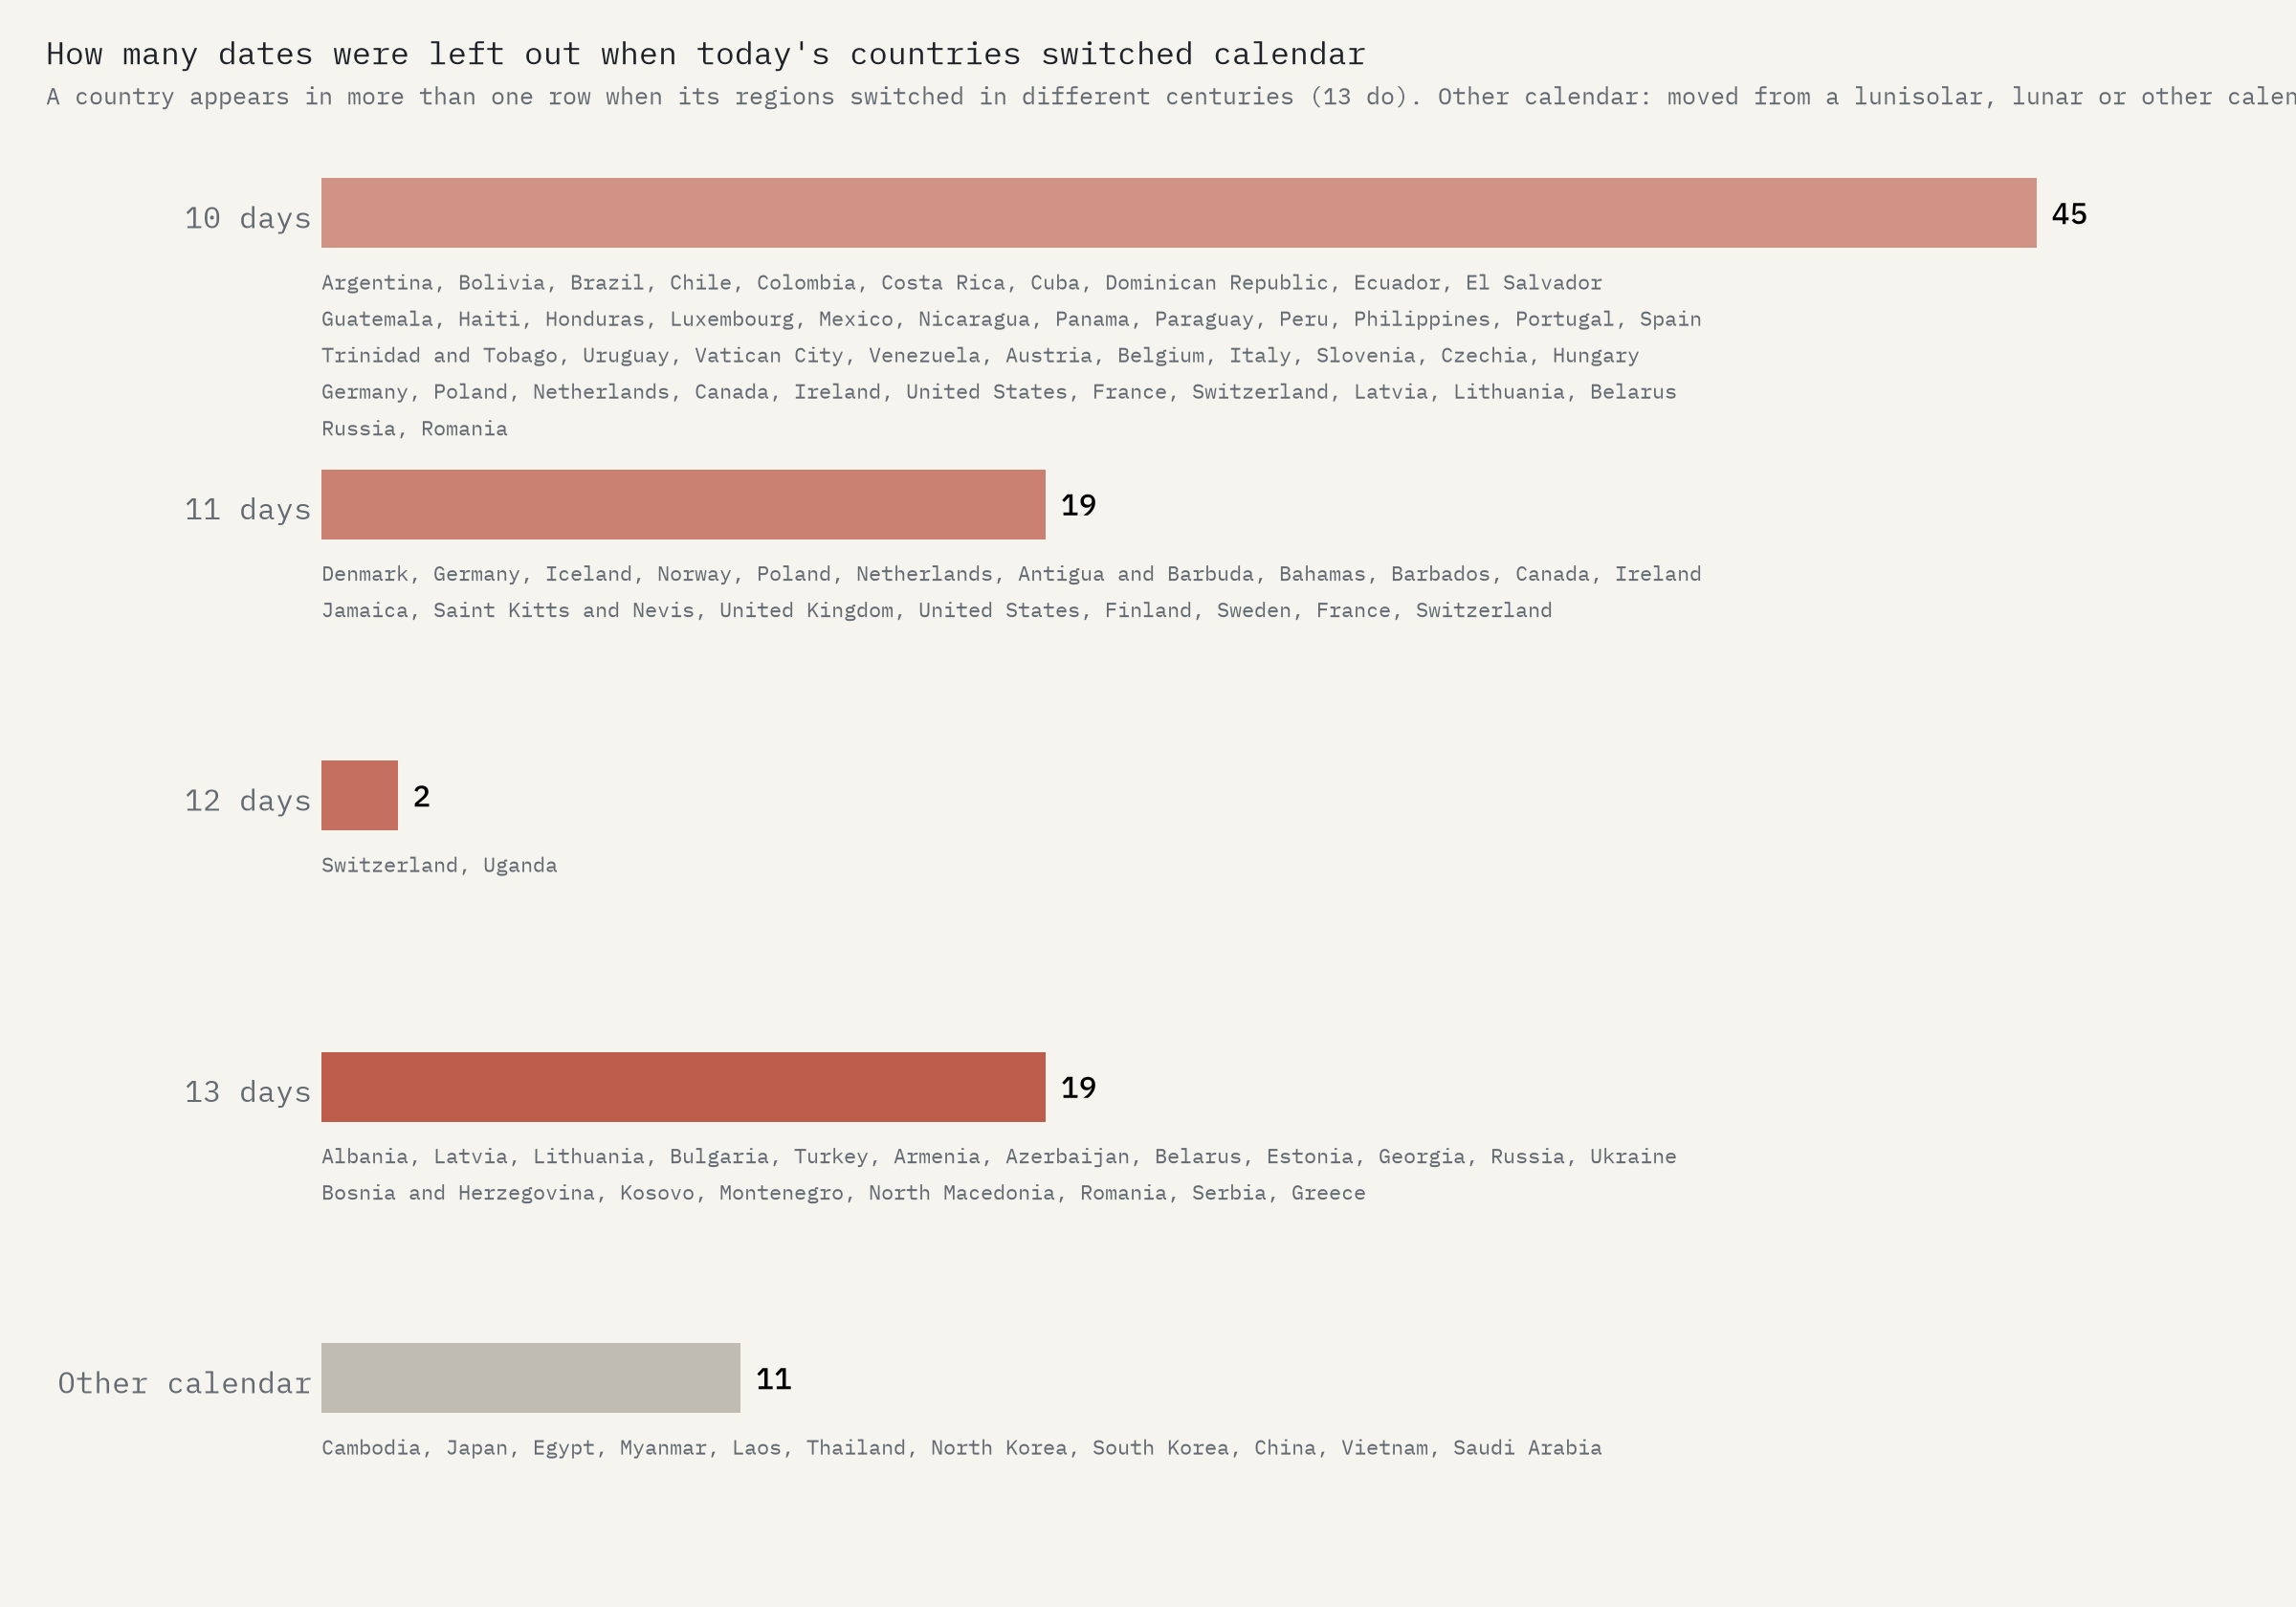
\includegraphics[width=\textwidth]{f_days.png}
\caption{Today's countries by the number of dates dropped at the switch.}\label{fig:days}\end{figure}

\subsection{Driving side}
The table records 62 of today's countries changing side at a known date (Figure~\ref{fig:roadsw}), 52 of them between 1919 and 1986, which matches the article's statement that 34 territories switched from left to right in that period only loosely, since the table and the statement count different units. The busiest decade was the 1920s (16 switches), with the states that emerged from Austria-Hungary, Italy, Spain, Portugal and its colonies; 20 switches came after 1960, mostly former British colonies joining right-hand neighbours. Only Namibia (1920), Timor-Leste (1976) and Samoa (2009) moved to the left. Today 54 countries drive on the left (Figure~\ref{fig:roadmap}); in Europe only Cyprus, Ireland, Malta and the United Kingdom.

\begin{figure}[tbp]\centering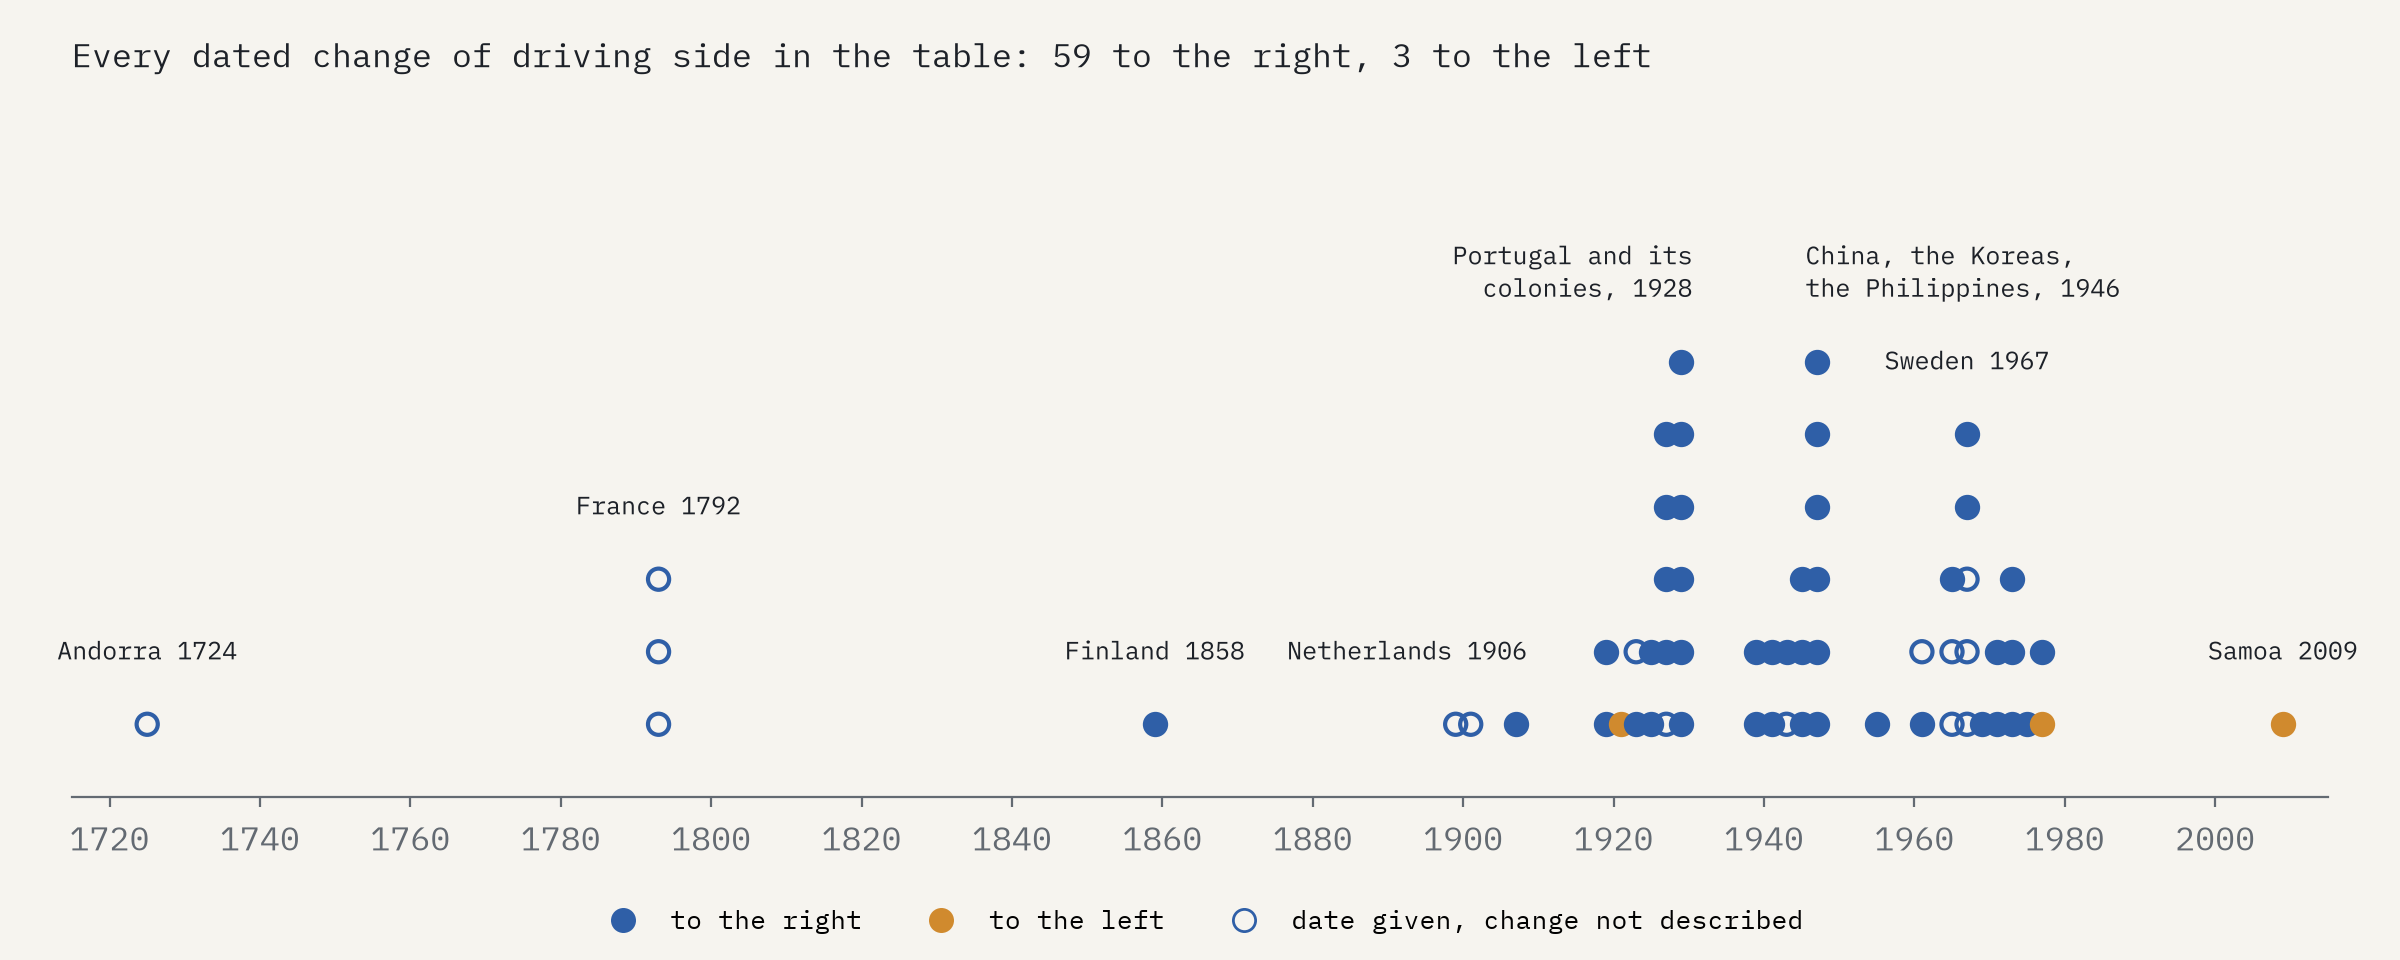
\includegraphics[width=\textwidth]{f_road_switches.png}
\caption{Every dated change of driving side in the table. Hollow: a date with no description of the change.}\label{fig:roadsw}\end{figure}

\begin{figure}[tbp]\centering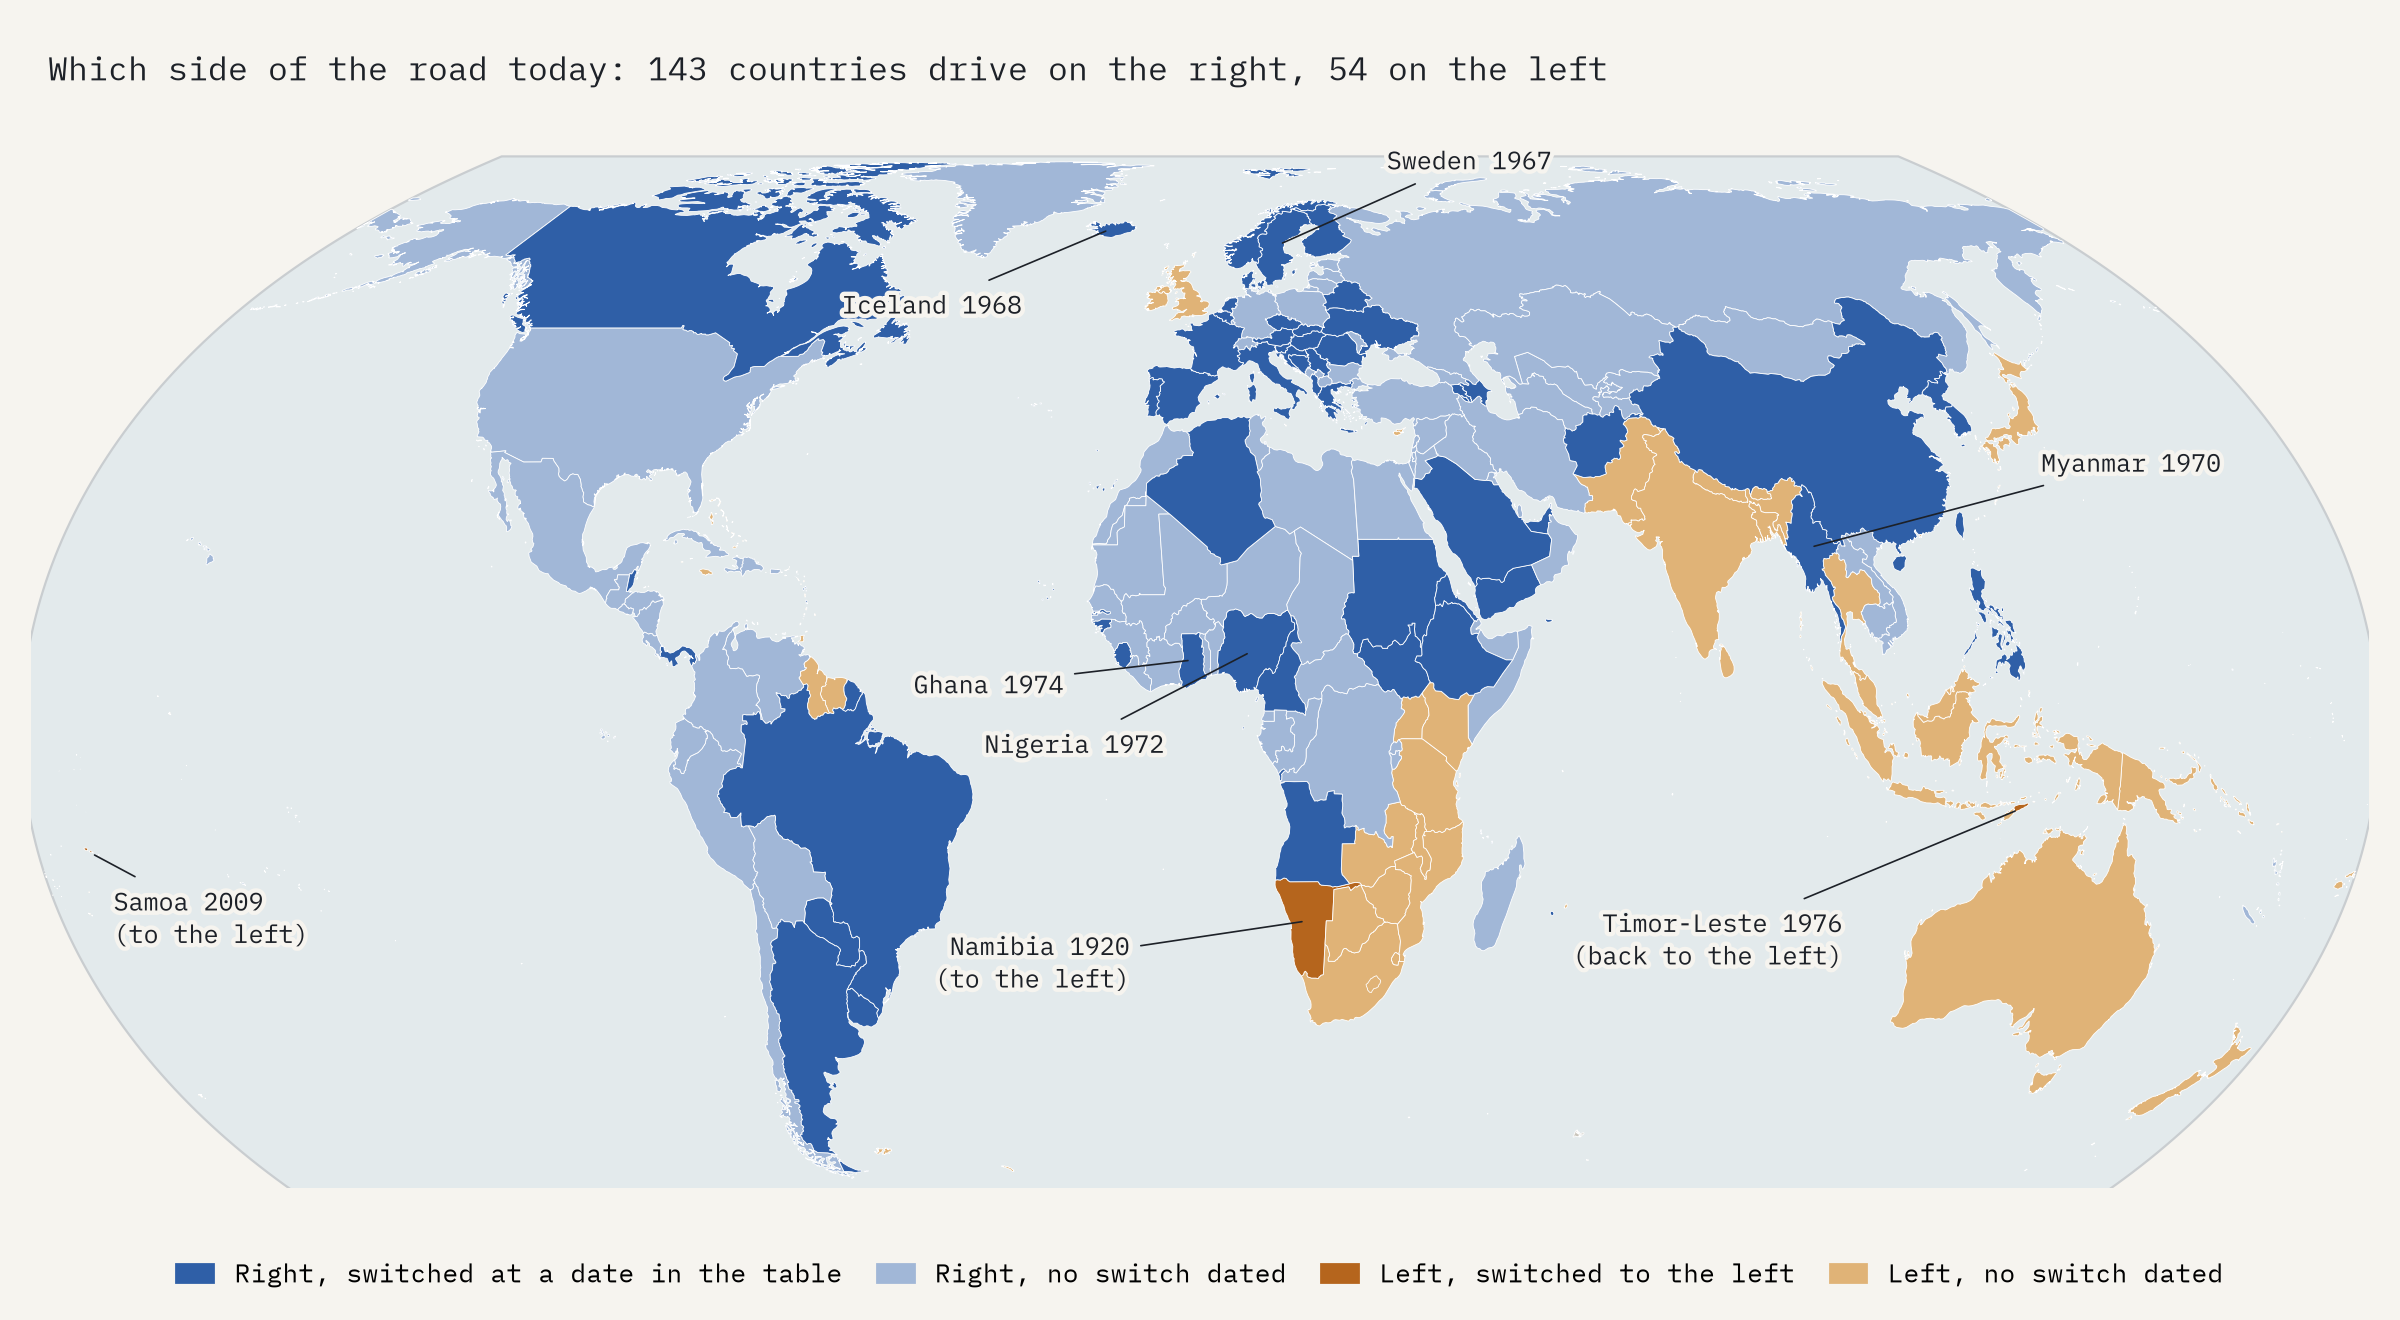
\includegraphics[width=\textwidth]{f_road_map.png}
\caption{Driving side today, distinguishing countries with a dated switch.}\label{fig:roadmap}\end{figure}

\begin{table}[tbp]\centering\footnotesize\setlength{\tabcolsep}{4pt}\caption{Every dated change of driving side in the table, matched to today's countries.}\label{tab:road}\begin{tabular}{lrl@{\hspace{1.4em}}lrl}\toprule Country & Year & To & Country & Year & To\\\midrule
Andorra & 1724 & right & Panama & 1943 & right\\
France & 1792 & right & Argentina & 1945 & right\\
Denmark & 1793 & right & Paraguay & 1945 & right\\
Norway & 1793 & right & Uruguay & 1945 & right\\
Finland & 1858 & right & China & 1946 & right\\
Belgium & 1899 & right & North Korea & 1946 & right\\
Algeria & 1900 & right & Philippines & 1946 & right\\
Netherlands & 1906 & right & South Korea & 1946 & right\\
Bosnia and Herzegovina & 1918 & right & Taiwan & 1946 & right\\
Romania & 1919 & right & Canada & 1947 & right\\
Namibia & 1920 & left & Afghanistan & 1955 & right\\
Ukraine & 1922 & right & Belize & 1961 & right\\
Armenia & 1923 & right & Cameroon & 1961 & right\\
Italy & 1924 & right & Eritrea & 1964 & right\\
Spain & 1924 & right & Ethiopia & 1964 & right\\
Albania & 1926 & right & Gambia & 1965 & right\\
Croatia & 1926 & right & Azerbaijan & 1966 & right\\
Greece & 1926 & right & Belarus & 1966 & right\\
Serbia & 1926 & right & United Arab Emirates & 1966 & right\\
Slovenia & 1926 & right & Bahrain & 1967 & right\\
Angola & 1928 & right & Sweden & 1967 & right\\
Brazil & 1928 & right & Iceland & 1968 & right\\
Cape Verde & 1928 & right & Myanmar & 1970 & right\\
Guinea-Bissau & 1928 & right & Sierra Leone & 1971 & right\\
Portugal & 1928 & right & Nigeria & 1972 & right\\
São Tomé and Príncipe & 1928 & right & South Sudan & 1973 & right\\
Austria & 1938 & right & Sudan & 1973 & right\\
Czechia & 1939 & right & Ghana & 1974 & right\\
Hungary & 1941 & right & Timor-Leste & 1976 & left\\
Slovakia & 1941 & right & Yemen & 1977 & right\\
Saudi Arabia & 1942 & right & Samoa & 2009 & left\\
\bottomrule\end{tabular}\end{table}

\subsection{Metrication}
Figure~\ref{fig:metric} maps the start of metrication for the 73 countries the table and prose date. 29 started in the nineteenth century, led by France (1795), Portugal (1814) and the Low Countries (1820). The latest in the table are Samoa (2015), Myanmar (2011), Saint Lucia (2005) and Trinidad and Tobago (2004). The table lists five countries as using other units officially alongside metric: Canada, Liberia, Myanmar, United Kingdom and United States; according to NIST, as cited in the article, Liberia, Myanmar and the United States are the three countries without mandatory metric laws. The United Kingdom started in 1965 and stopped compulsory conversion in 1979; the United States made metric units lawful in 1866 without displacing customary units.

\begin{figure}[tbp]\centering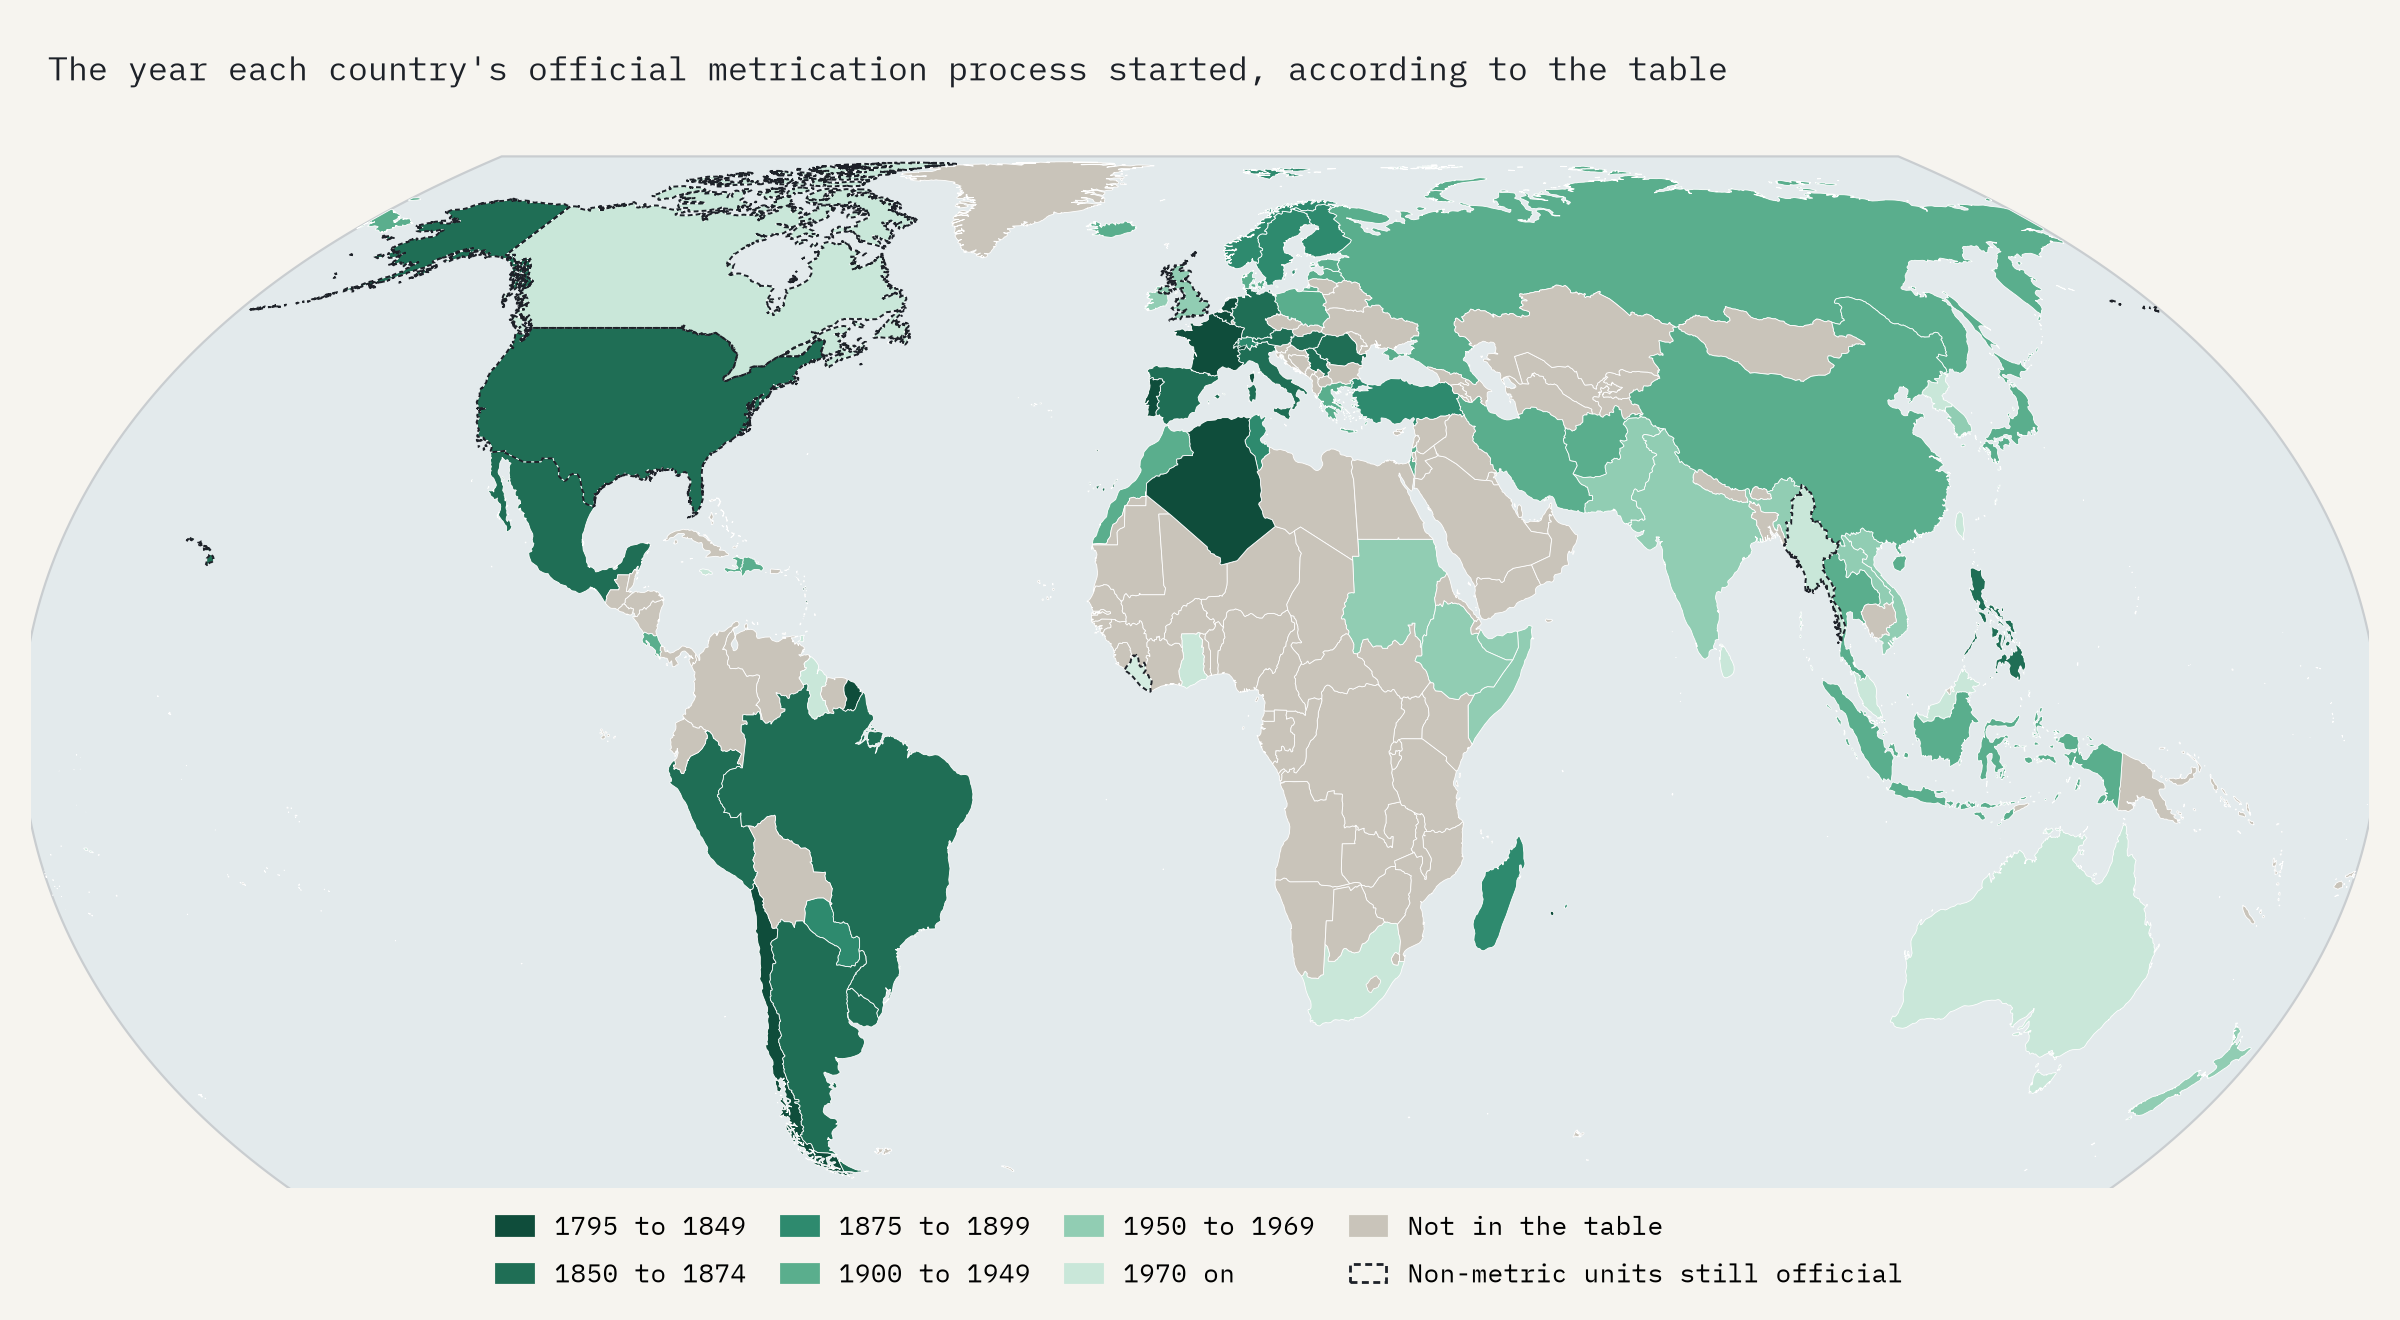
\includegraphics[width=\textwidth]{f_metric_map.png}
\caption{The year each country's official metrication process started. Dashed: non-metric units still official.}\label{fig:metric}\end{figure}

\subsection{Votes for women}
Figure~\ref{fig:vote} maps the first national vote. New Zealand (1893) was first, followed by Australia (1902, with racial exclusions until 1962), Finland (1906) and Norway (1913). The busiest decade was the 1950s (42 countries), and 81 countries first gave women the vote in the 1940s and 1950s. The latest were Saudi Arabia (2015, municipal elections only), United Arab Emirates (2006), Kuwait (2005), Oman and Bahrain (2002) and Qatar (1997). Switzerland's federal vote came in 1971 and Appenzell Innerrhoden's cantonal vote in 1990. Table~\ref{tab:votes} and Figure~\ref{fig:two} show the 18 countries with a separate year for equal or full terms; the gap ranges from one year (Moldova) to 65 (Portugal; 64 in South Africa). Portugal's vote, granted with restrictions in 1911, was withdrawn and restored in 1931 before becoming unrestricted in 1976.

\begin{figure}[tbp]\centering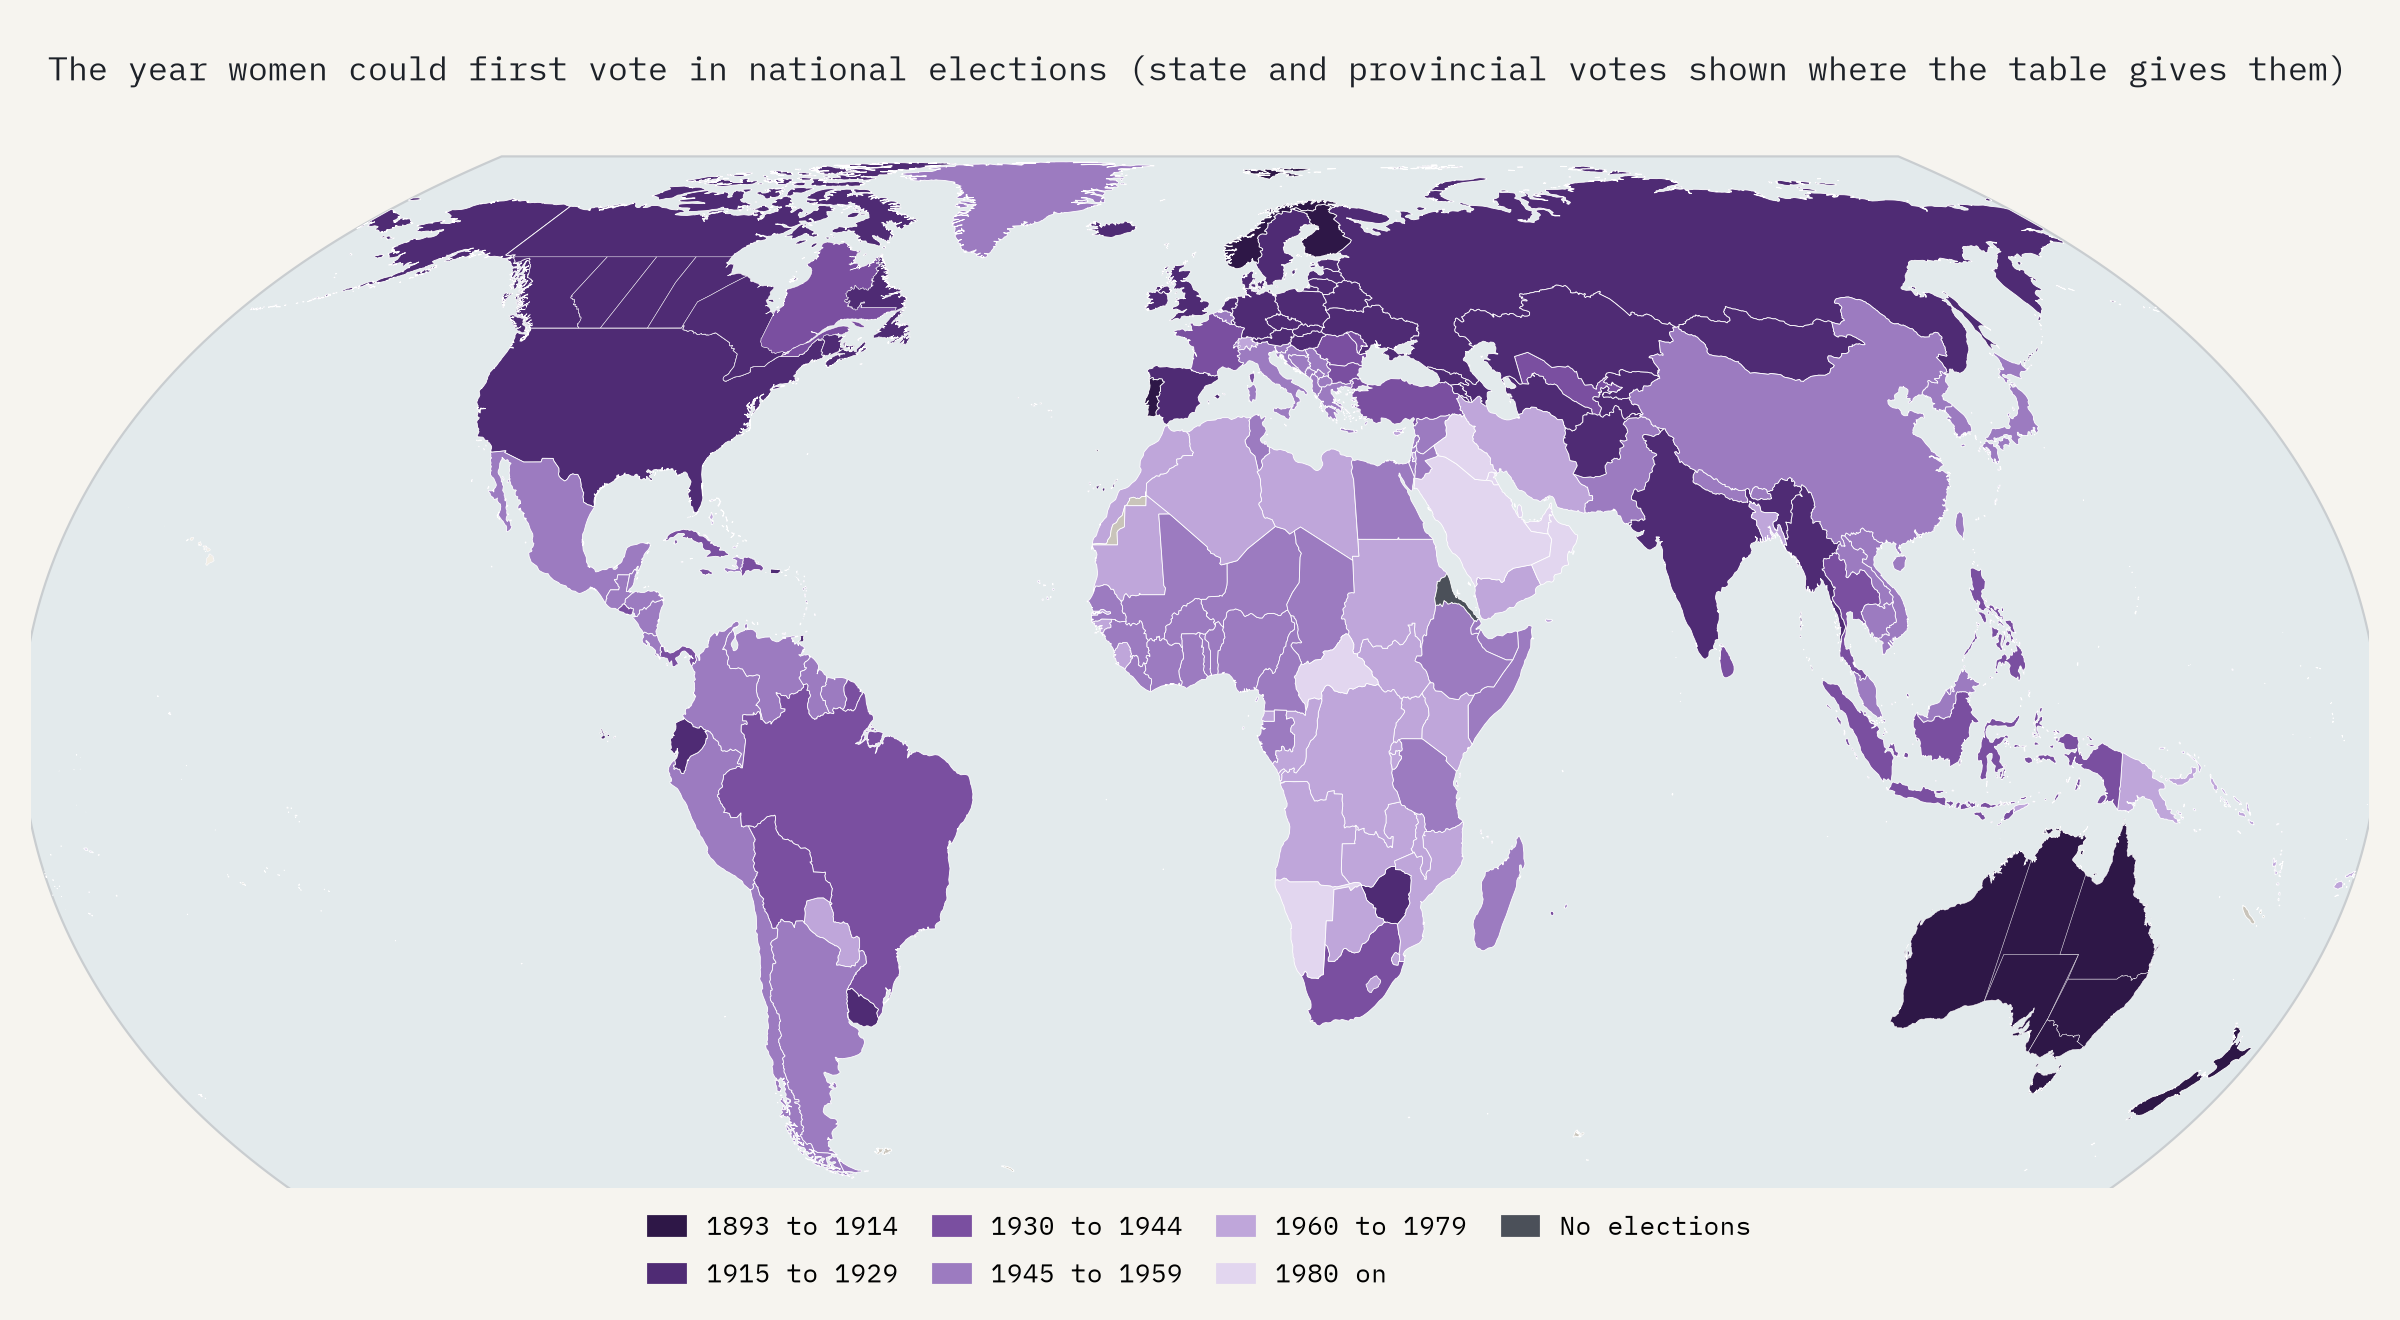
\includegraphics[width=\textwidth]{f_vote_map.png}
\caption{The year women could first vote in national elections.}\label{fig:vote}\end{figure}

\begin{figure}[tbp]\centering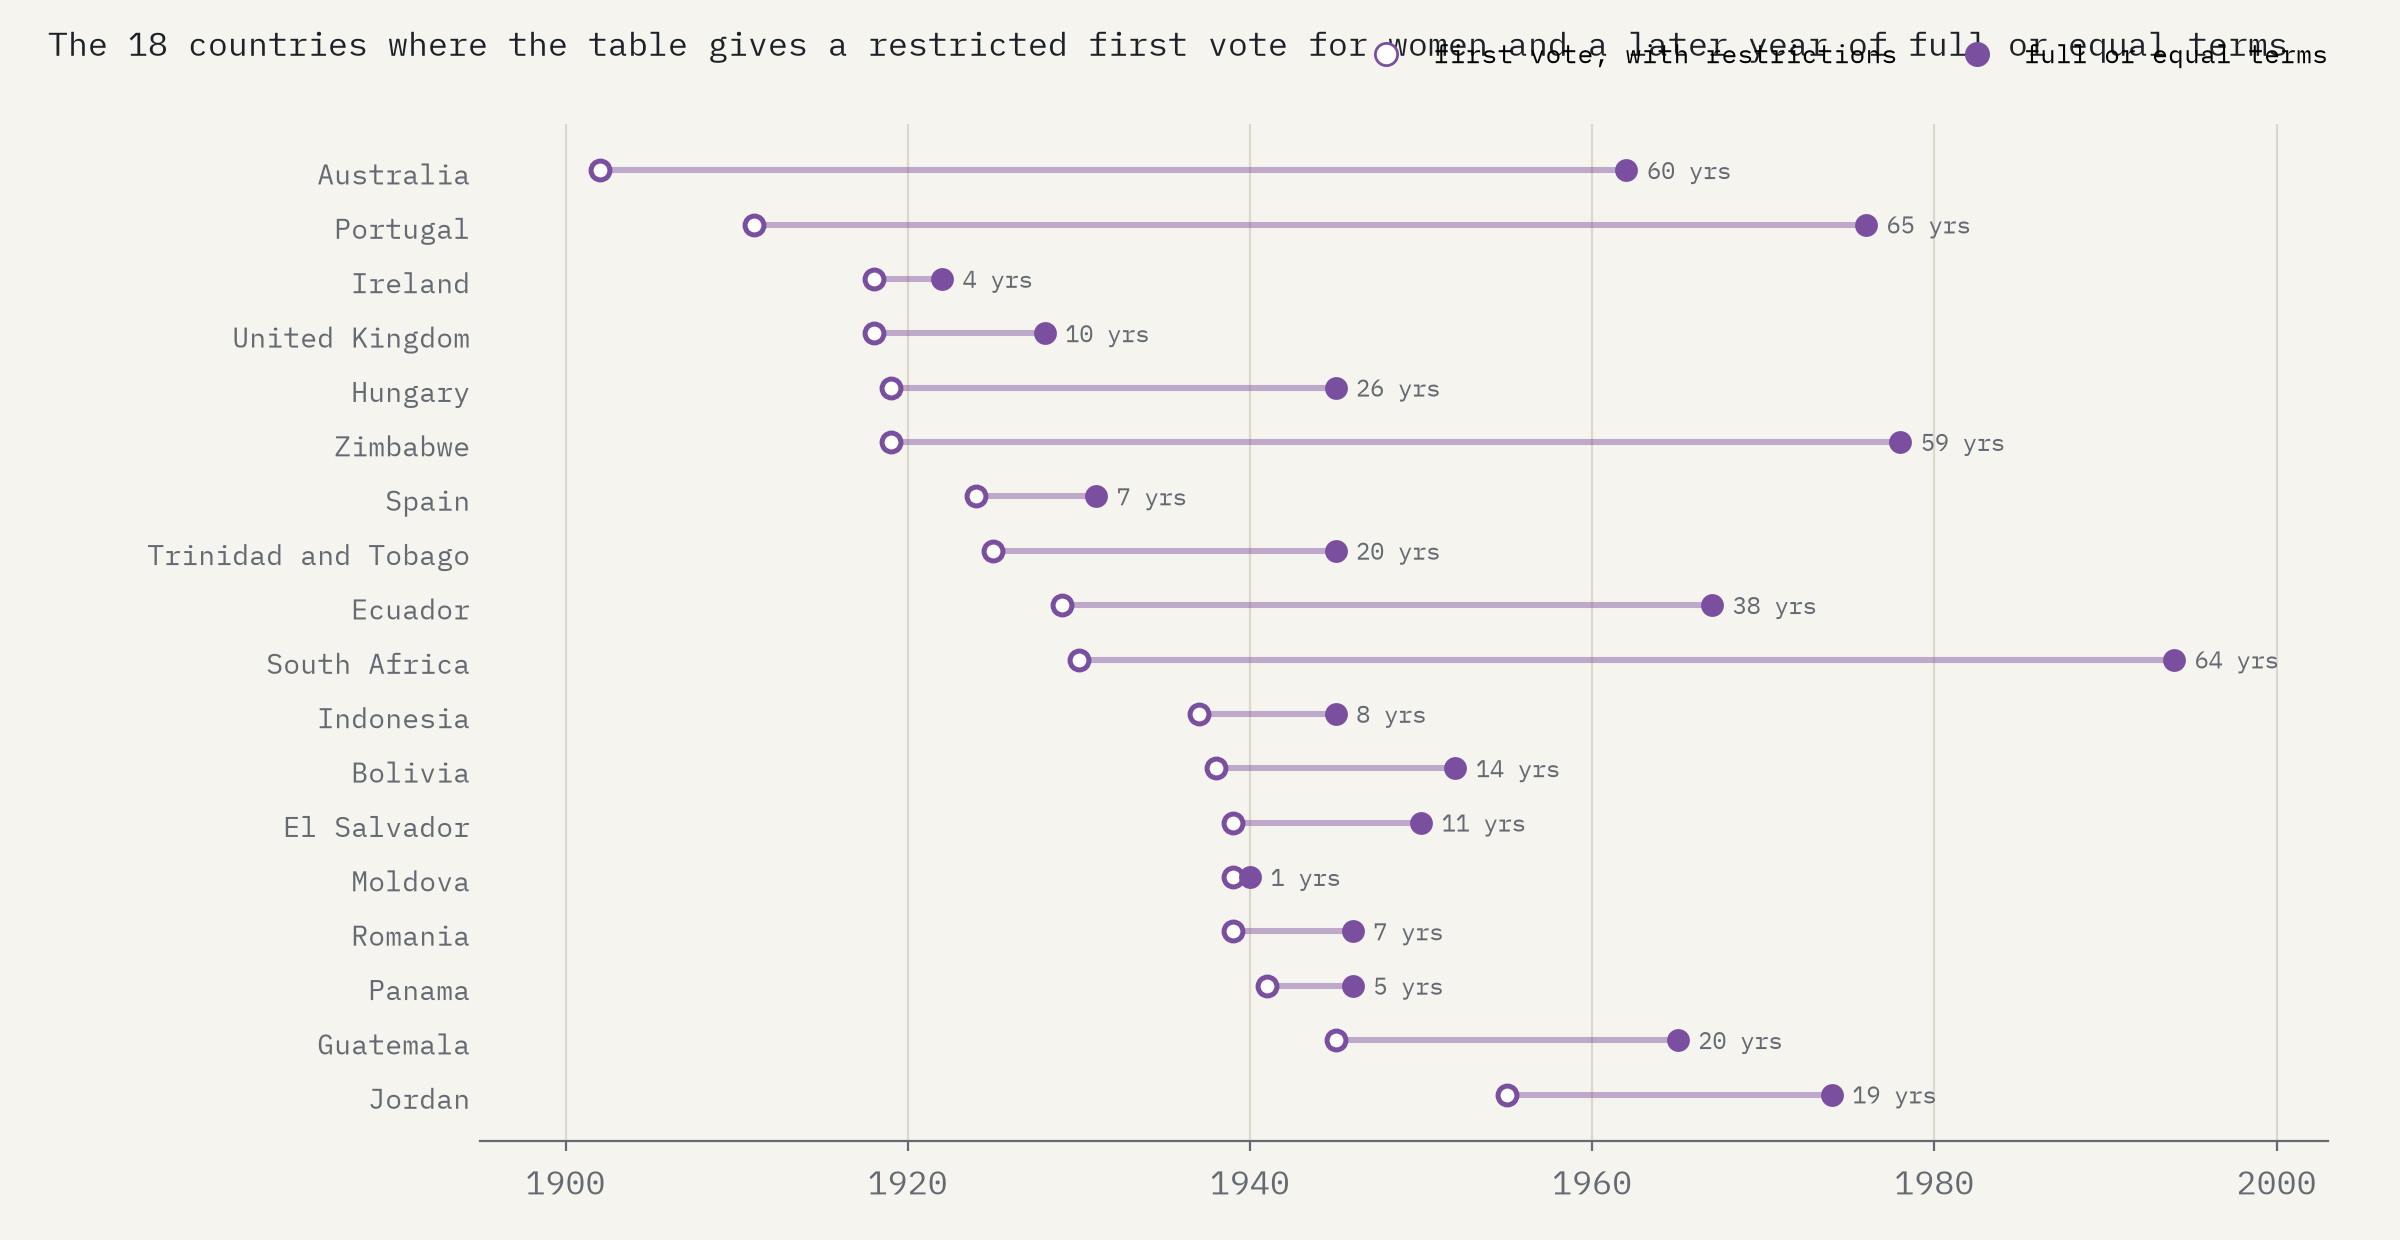
\includegraphics[width=\textwidth]{f_vote_two.png}
\caption{First (restricted) and full or equal votes for women, where the table gives both.}\label{fig:two}\end{figure}

\begin{table}[tbp]\centering\footnotesize\caption{Countries where the suffrage table gives a restricted first vote and a later year of full or equal terms, with my reading of the table.}\label{tab:votes}\begin{tabular}{lrrp{9.6cm}}\toprule Country & First & Equal & Reading of the table\\\midrule
Australia & 1902 & 1962 & 1902 at federal level except for 'natives of Australia, Asia, Africa and the Pacific Islands'; 1962 full.\\
Portugal & 1911 & 1976 & 1911 with restrictions, then made illegal again until 1931, when it returned with restrictions; restrictions other than age lifted in 1976.\\
Ireland & 1918 & 1922 & 1918 at 30 with property qualifications, as in the rest of the United Kingdom; equal in the Irish Free State from 1922.\\
United Kingdom & 1918 & 1928 & 1918 at 30 with property qualifications or as graduates, while men voted at 21; equal from 1928.\\
Hungary & 1919 & 1945 & 1919 from age 30 with higher criteria than men (men from 24); universal from age 20 for both in 1945.\\
Zimbabwe & 1919 & 1978 & 1919 for white women only; full in 1978.\\
Spain & 1924 & 1931 & Women briefly held the vote from 1924 to 1926 but no elections were held; the 1931 constitution gave the vote, first used in 1933; nobody voted again until after Franco.\\
Trinidad and Tobago & 1925 & 1945 & 1925 for women over 30 (men over 21), as in the United Kingdom; full suffrage in 1945.\\
Ecuador & 1929 & 1967 & 1929, but voting was optional for women and compulsory for men until 1967.\\
South Africa & 1930 & 1994 & 1930 for European and Asian women; women of other races in 1994, at the same time as men of all races.\\
Indonesia & 1937 & 1945 & 1937 for Europeans only; 1945 for all citizens, at independence.\\
Bolivia & 1938 & 1952 & 1938 for literate women with an income; equal with men from 1952.\\
El Salvador & 1939 & 1950 & 1939 with literacy and higher age requirements; all restrictions lifted in 1950.\\
Moldova & 1939 & 1940 & 1929 local elections as part of Romania; general elections from the 1939 electoral law; equal in 1940 in the Moldavian SSR.\\
Romania & 1939 & 1946 & 1929 in local elections with qualifications; general elections under the 1939 electoral law, with restrictions that weighed more on women; full equality in 1946.\\
Panama & 1941 & 1946 & 1941 conditioned by education; equal from 1946.\\
Guatemala & 1945 & 1965 & 1945 for literate women; restrictions lifted in 1965.\\
Jordan & 1955 & 1974 & 1955 for educated women; all women in 1974.\\
\bottomrule\end{tabular}\end{table}

\subsection{Holdouts}
The United Kingdom is a holdout across switches: it adopted the calendar 170 years after Rome, drives on the left, began metrication only in 1965 and halted it in 1979, and gave women the vote on equal terms ten years after the first, restricted vote. The Gulf monarchies were the last for votes; the Orthodox east and Turkey the last in Europe for the calendar; the former British colonies of West Africa among the last to change side.

\section{Limitations}
First, Wikipedia's tables are compiled by many contributors, several cells are flagged as needing citations, and I have not checked them against primary sources. Second, the calendar record is incomplete: even with the list, 111 countries, including India, Indonesia, Pakistan and most of Africa, have no date, though they use the Gregorian calendar today; the list concentrates on Europe and on places that came from the Julian calendar. The same is true of metrication for 120 countries. Third, the colonial mapping for the calendar and the stand ins for historical states are my decisions. Fourth, for driving, the assumption that undated countries always used today's side is not supported by the sources and certainly fails for some. Fifth, the vote years mix legal grant and first exercise as the table does, and the national level hides federal and local differences. Sixth, population weights are today's.

\section{Conclusion}
Four centuries of switching produced near agreement on the calendar, the vote and, in law if not in practice, the metre; the side of the road settled with nearly three quarters of countries on the right. The waves followed the religious map of Europe, the reach of empires, the two world wars and decolonisation. The stragglers are informative: religious calendars kept for faith, island nations and former British colonies keeping left, and states where rights to vote were granted last or not at all.

\section*{Data and code availability}
The interactive map is at \url{https://maps.tristanhotham.com/calendar-switch/}. Data and code are at \url{https://github.com/Tristan-Hotham/calendar-switch} and archived with this paper at https://doi.org/10.5281/zenodo.23873009. Code is released under the MIT licence; text and figures under CC BY 4.0; the tables derived from Wikipedia under CC BY-SA 4.0.

\section*{AI statement}
I wrote the text, with drafting and editing assistance from Claude (Anthropic), which also helped prepare the analysis code. I reviewed and checked all text and results.

\begin{table}[tbp]\centering\small\caption{English Wikipedia articles used, with the revision read (CC BY-SA 4.0).}\label{tab:revs}\begin{tabular}{lr}\toprule Article & Revision\\\midrule
Adoption of the Gregorian calendar & 1377458140\\
Calendar (New Style) Act 1750 & 1381810314\\
Coordinated Universal Time & 1382958828\\
Dagen H & 1376222830\\
Daylight saving time by country & 1382749307\\
Decimalisation & 1376953205\\
Gregorian calendar & 1380886632\\
Julian calendar & 1382567429\\
Left- and right-hand traffic & 1382823315\\
List of adoption dates of the Gregorian calendar by country & 1362271356\\
Metric system & 1380041985\\
Metrication & 1382862581\\
Old Style and New Style dates & 1380273862\\
Revised Julian calendar & 1383288345\\
Time zone & 1380240509\\
Timeline of women's legal rights (other than voting) & 1382726829\\
Timeline of women's suffrage & 1379988760\\
Universal suffrage & 1357310178\\
Women's suffrage & 1382653198\\
\bottomrule\end{tabular}\end{table}

\begin{thebibliography}{9}
\bibitem[Natural Earth(2026)]{naturalearth} Natural Earth (2026) Admin 0 countries (1:50m) and admin 1 states and provinces (1:10m). Public domain. \url{https://www.naturalearthdata.com/}
\bibitem[Wikipedia(2026)]{wiki} Wikipedia contributors (2026) English Wikipedia articles listed in Table~\ref{tab:revs}, at the revisions given. CC BY-SA 4.0. \url{https://en.wikipedia.org/}
\end{thebibliography}
\end{document}
